\documentclass[11pt]{article}
\usepackage[a4paper,margin=1in]{geometry}
\usepackage[T1]{fontenc}
\usepackage{lmodern}
\usepackage{microtype}
\usepackage{amsmath,amssymb,amsthm}
\usepackage{booktabs,tabularx,array}
\usepackage{enumitem}
\usepackage{xcolor}
\usepackage{listings}
\usepackage{xurl}
\usepackage{tikz}
\usetikzlibrary{positioning,arrows.meta,fit}
\usepackage[colorlinks=true,linkcolor=blue!50!black,urlcolor=blue!50!black]{hyperref}

\setlist{itemsep=2pt,topsep=4pt}
\lstset{basicstyle=\ttfamily\small,columns=fullflexible,keepspaces=true,
  frame=single,framerule=0.3pt,xleftmargin=4pt,xrightmargin=4pt,
  aboveskip=8pt,belowskip=8pt,showstringspaces=false,breaklines=true}
\colorlet{fg}{black}
\newcommand{\kw}[1]{\texttt{#1}}
\theoremstyle{definition}
\newtheorem{obligation}{Obligation}
\renewcommand{\theobligation}{P\arabic{obligation}}

\title{From Cloud Build to Running Hardware\\[4pt]
\large Development specification: build host, relay, and Kria KV260 target\\
for the hardware rendering of the rho calculus}
\author{F1R3FLY.io design note --- draft 0.1}
\date{13 November 2026}

\begin{document}
\maketitle
\begin{abstract}
\noindent
This note specifies the path a build takes from source to running hardware
for the rho hardware rendering: a rented cloud instance builds the
bitstream, an iMac relays it and serves as the terminal, and an AMD Kria
KV260 runs it. It fixes the roles of the three machines, the artifacts that
cross between them, the board-support wrapper that the tile array needs on
this board, the packaging and loading procedure, the checks that establish
that the hardware under test is the hardware that was built, and a bring-up
ladder. It is a companion to the design specification (draft 0.5) and
changes nothing in it. Nothing here has yet been run on a board; every
decision is marked proposed, and Section~\ref{sec:open} lists what the first
bring-up has to settle.

\end{abstract}
\tableofcontents
%======================================================================
\section{Purpose and scope}

The design specification says what the machine is. This note says how a
change to the Bluespec source becomes a running array of tiles on a board,
and how the evidence of what the array did gets back to the checker. Three
constraints shape it.
\begin{itemize}
\item The vendor tools for this board run on x86-64 Linux or Windows and not
on macOS, so builds happen on a rented cloud instance.
\item The board sits on a local network behind a router, so the cloud
instance cannot reach it. The iMac can reach both.
\item The verification obligations of the design specification are stated
over decision logs. A log is evidence only if the bitstream that produced it
is known to be the one that was built from the source under review.
\end{itemize}
In scope: the three machines and their roles, the artifacts, the
board-support wrapper, packaging, transfer, loading, log return, and the
checks on the path itself. Out of scope: the machine (design specification),
the f1r3lang compiler, and timing closure for any particular array size.

%======================================================================
\section{Roles and topology}\label{sec:roles}

\begin{figure}[h]
\centering
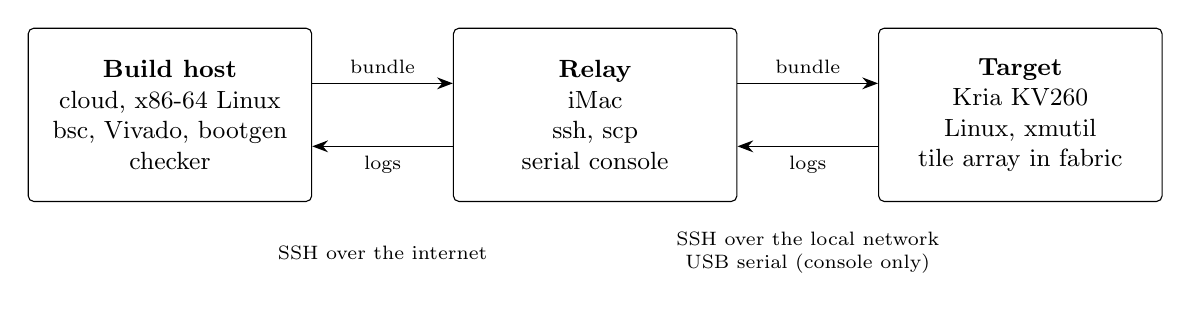
\begin{tikzpicture}[
  box/.style={draw=fg,rounded corners=2pt,minimum width=36mm,minimum height=22mm,
              align=center,font=\small},
  arr/.style={-{Stealth[length=2mm]},semithick,draw=fg},
  lab/.style={font=\scriptsize,align=center}]
\node[box] (cloud) at (0,0) {\textbf{Build host}\\cloud, x86-64 Linux\\bsc, Vivado, bootgen\\checker};
\node[box] (mac) at (5.4,0) {\textbf{Relay}\\iMac\\ssh, scp\\serial console};
\node[box] (kria) at (10.8,0) {\textbf{Target}\\Kria KV260\\Linux, xmutil\\tile array in fabric};
\draw[arr] ([yshift=4mm]cloud.east) -- node[lab,above] {bundle} ([yshift=4mm]mac.west);
\draw[arr] ([yshift=4mm]mac.east) -- node[lab,above] {bundle} ([yshift=4mm]kria.west);
\draw[arr] ([yshift=-4mm]kria.west) -- node[lab,below] {logs} ([yshift=-4mm]mac.east);
\draw[arr] ([yshift=-4mm]mac.west) -- node[lab,below] {logs} ([yshift=-4mm]cloud.east);
\node[lab] at (2.7,-1.75) {SSH over the internet};
\node[lab] at (8.1,-1.75) {SSH over the local network\\USB serial (console only)};
\end{tikzpicture}
\caption{The three machines. The iMac opens both connections; neither end
connects to the other.}
\end{figure}

\begin{center}
\begin{tabularx}{\linewidth}{@{}l X X@{}}
\toprule
Machine & Does & Does not\\
\midrule
Build host & Compiles Bluespec to Verilog, simulates, synthesises, places and
routes, packages the bundle, runs the checker over returned logs &
Reach the board\\
Relay (iMac) & Starts builds over SSH, copies the bundle across, opens the
shell and the serial console on the board, flashes the SD card once &
Run any vendor tool; drive JTAG\\
Target (Kria) & Loads the bundle into the fabric at run time, loads images,
runs, drains decision logs to files & Build anything\\
\bottomrule
\end{tabularx}
\end{center}

Because the relay runs no vendor tool, its processor architecture does not
matter. The question of Intel or Apple silicon, open in the board
discussion, is closed by this arrangement.

%======================================================================
\section{Decision register}\label{sec:decisions}

All decisions are proposed by this draft. They are numbered B1 onward to
keep them apart from D1 to D32 of the design specification.

\begin{center}
\begin{tabularx}{\linewidth}{@{}l X@{}}
\toprule
 & Decision\\
\midrule
B1 & Builds run on a cloud x86-64 Linux instance, started for a build and
stopped afterwards.\\
B2 & The bitstream is loaded at run time from the board's own Linux with
\kw{xmutil}; no JTAG cable and no boot-image rebuild is part of the normal
loop.\\
B3 & The relay pulls from the build host and pushes to the target. No
inbound connection to the local network is opened. An overlay network
(Section~\ref{sec:transfer}) is an allowed alternative, not the default.\\
B4 & The tile array is wrapped in a board-support module with one AXI4-Lite
slave, clocked and reset by the processor block. The wrapper is the only
board-specific RTL.\\
B5 & The wrapper is written in Bluespec, like the rest of the design, with
no external AXI library.\\
B6 & Every bitstream carries a build identity (source revision, build time,
array dimensions) readable from the register interface.\\
B7 & Every bundle carries a manifest of SHA-256 digests, checked on the
target before loading.\\
B8 & When the log buffer is nearly full the array stalls by clock enable; it
never drops a log record.\\
B9 & Log readout is by register access for stages L1 to L3
(Section~\ref{sec:ladder}); a streaming path replaces it only when measured
throughput requires.\\
B10 & The device tree overlay is generated from the hardware description
exported by the build, not written by hand.\\
\bottomrule
\end{tabularx}
\end{center}

%======================================================================
\section{Artifacts}\label{sec:artifacts}

A \emph{bundle} is a directory named for the application; the name used
throughout is \kw{rho}. The loader on the target requires three files: the
bitstream in \kw{.bit.bin} form, a device tree overlay, and a
\kw{shell.json} descriptor. The bitstream and the overlay share a base name.
This note adds a fourth file, the manifest.

\begin{center}
\begin{tabularx}{\linewidth}{@{}l l X@{}}
\toprule
File & Made by & Content\\
\midrule
\kw{rho.bit.bin} & Vivado, then bootgen & The fabric configuration with the
bitstream header stripped\\
\kw{rho.dtbo} & device tree generator, then \kw{dtc} & Overlay naming the
bitstream, enabling the fabric clock, and declaring the register region\\
\kw{shell.json} & fixed text & Descriptor for the loader: a flat design with
one slot\\
\kw{MANIFEST} & build script & Build identity and the SHA-256 digest of each
of the other three files\\
\bottomrule
\end{tabularx}
\end{center}

Images (compiled programs for the array, in the image format of the design
specification) and decision logs are not part of the bundle. Images travel
the same route in the same direction; logs travel it in reverse.

%======================================================================
\section{Build host}\label{sec:build}

\subsection{Instance}
An x86-64 Linux instance on a distribution the installed Vivado version
supports. A starting size of 8 virtual CPUs, 32 GB of memory and 150 GB of
disk is proposed; the disk is dominated by the Vivado installation. The
device on the Kria K26 module is in the set that the no-cost Vivado edition
covers, to be confirmed against the licence terms of the version installed.
Inbound access is SSH only, by key, restricted to the address of the relay.
The instance is stopped when no build is running; its disk persists.

\subsection{Tools}
\begin{itemize}
\item \kw{bsc}, the Bluespec compiler, release 2026.07.1 (the version
already exercised for this project).
\item Icarus Verilog, for simulation of the generated Verilog before any
synthesis is attempted.
\item Vivado, with \kw{bootgen} and the device tree generator that ship
with it.
\item \kw{dtc}, the device tree compiler.
\item GHC, to build \kw{rhoref} and its checker.
\end{itemize}

\subsection{Repository layout}
\begin{lstlisting}
rho-hw/
  bsv/            Bluespec source: tile, mesh, array, board wrapper
  rhoref/         reference implementation and checker
  board/kv260/    build.tcl, shell.json
  scripts/        build.sh, package.sh
  build/          generated; never committed
    verilog/      output of bsc
    vivado/       project, reports, rho.bit, system.xsa
    bundle/rho/   the four files of Section 4
\end{lstlisting}

\subsection{Build steps}\label{sec:steps}
\begin{enumerate}
\item \textbf{Identity.} Record the source revision and the build time; refuse
to produce a release bundle from a working tree with uncommitted changes.
\item \textbf{Compile.} Run \kw{bsc -verilog} on the board wrapper as the
top module, with the array dimensions and the identity as parameters.
\item \textbf{Simulate.} Run the generated Verilog under Icarus against the
directed programs of the design specification and compare logs with
\kw{rhoref}. A failure here stops the build; synthesis time is not spent on
a design that fails simulation.
\item \textbf{Synthesise and implement.} Run Vivado in batch mode on
\kw{build.tcl}. Sources are the generated Verilog and the Verilog primitives
that \kw{bsc} ships for Vivado. A build that does not meet timing fails; no
bundle is produced.
\item \textbf{Export.} Write \kw{rho.bit} and the hardware description
\kw{system.xsa}. Keep the utilisation and timing reports beside them.
\item \textbf{Package.} Produce the bundle (Section~\ref{sec:package}).
\end{enumerate}

The Tcl below is a sketch of step 4, to be made exact against the installed
Vivado version at first bring-up.
\begin{lstlisting}
create_project rho_kv260 build/vivado -part xck26-sfvc784-2LV-c
set_property board_part [get_board_parts *kv260_som*] [current_project]
add_files [glob build/verilog/*.v]
create_bd_design system
create_bd_cell -type ip -vlnv xilinx.com:ip:zynq_ultra_ps_e ps
apply_bd_automation -rule xilinx.com:bd_rule:zynq_ultra_ps_e \
    -config {apply_board_preset 1} [get_bd_cells ps]
create_bd_cell -type module -reference mkRhoBoard rho
# connect the AXI4-Lite slave to the processor block, with clock and reset
apply_bd_automation -rule xilinx.com:bd_rule:axi4 \
    -config {Master /ps/M_AXI_HPM0_FPD Clk Auto} [get_bd_intf_pins rho/s_axi]
make_wrapper -files [get_files system.bd] -top -import
launch_runs impl_1 -to_step write_bitstream -jobs 8
wait_on_run impl_1
write_hw_platform -fixed -include_bit build/vivado/system.xsa
\end{lstlisting}

%======================================================================
\section{Board-support wrapper}\label{sec:wrapper}

On this board the fabric has no oscillator of its own in the path used here:
clock and reset come from the processor block. The top level is therefore
not the tile array but a wrapper, \kw{mkRhoBoard}, containing the array and
one AXI4-Lite slave.

\subsection{Clock, reset, stall}
\begin{itemize}
\item One clock domain, driven by the first fabric clock of the processor
block. Its frequency is a build parameter, chosen after the first tile has
been synthesised.
\item Reset is the processor block's fabric reset, synchronised in the
wrapper. A second, soft reset is a bit of the control register.
\item The array has a clock enable. It is deasserted while the run bit is
clear and while the log buffer is above its high-water mark (B8). The cycle
counter of the design specification counts enabled cycles, so a stall is
invisible to the logs and the replay obligation is unaffected.
\end{itemize}

\subsection{Register map}\label{sec:regs}
Registers are 32 bits wide. Offsets are from the base address that Vivado
assigns to the slave, which the overlay records. Wider machine words cross
as consecutive 32-bit accesses, low half first.

\begin{center}
\begin{tabularx}{\linewidth}{@{}l l l X@{}}
\toprule
Offset & Name & Access & Meaning\\
\midrule
\kw{0x00} & \kw{ID} & read & Constant \kw{0x52484F31}\\
\kw{0x04} & \kw{BUILD\_REV} & read & Source revision, first 32 bits\\
\kw{0x08} & \kw{BUILD\_TIME} & read & Build time, seconds since the epoch\\
\kw{0x0C} & \kw{CONFIG} & read & Array width, array height, specification
draft\\
\kw{0x10} & \kw{CTRL} & write & Run, soft reset, single step\\
\kw{0x14} & \kw{STATUS} & read & Running, quiescent, fault, stalled\\
\kw{0x18} & \kw{CYCLE\_LO} & read & Enabled cycles, low half\\
\kw{0x1C} & \kw{CYCLE\_HI} & read & Enabled cycles, high half\\
\kw{0x20} & \kw{TILE\_SEL} & write & Tile addressed by the seed and image
registers\\
\kw{0x24} & \kw{SEED} & write & Arbiter seeds of the selected tile, in order\\
\kw{0x28} & \kw{IMG\_ADDR} & write & Image load address in the selected tile\\
\kw{0x2C} & \kw{IMG\_DATA} & write & Image word; the address then advances\\
\kw{0x30} & \kw{INGRESS} & write & Term-stream word into the array boundary\\
\kw{0x34} & \kw{EGRESS} & read & Term-stream word out of the boundary; a read
removes it\\
\kw{0x38} & \kw{IO\_LEVEL} & read & Free ingress space, pending egress words\\
\kw{0x3C} & \kw{LOG\_DATA} & read & Next log word; a read removes it\\
\kw{0x40} & \kw{LOG\_LEVEL} & read & Log words pending\\
\kw{0x44} & \kw{FAULT\_TILE} & read & Tile that raised the first fault\\
\kw{0x48} & \kw{FAULT\_CODE} & read & Fault code of the design specification\\
\kw{0x4C} & \kw{SCRATCH} & read, write & No effect; used to test the bus\\
\bottomrule
\end{tabularx}
\end{center}

The static code segment is replicated in every tile, so image loading
writes the same words to each tile in turn; a broadcast value of
\kw{TILE\_SEL} is reserved for that purpose. Image and seed writes are
accepted only while the run bit is clear.

%======================================================================
\section{Packaging}\label{sec:package}

\paragraph{Bitstream.} Strip the header with \kw{bootgen}:
\begin{lstlisting}
echo 'all:{rho.bit}' > bootgen.bif
bootgen -w -arch zynqmp -process_bitstream bin -image bootgen.bif
\end{lstlisting}
The result is \kw{rho.bit.bin}.

\paragraph{Overlay.} Generate the fabric device tree source from
\kw{system.xsa} with the device tree generator of the installed tool
version. In the generated source, set the firmware name to the name of the
packaged bitstream, then compile:
\begin{lstlisting}
firmware-name = "rho.bit.bin";

dtc -@ -O dtb -o rho.dtbo pl.dtsi
\end{lstlisting}
The generated overlay also enables the fabric clock and declares the
register region, which is why it is generated and not written by hand (B10).
The register region is bound to the generic user-space I/O driver, so the
tools on the target reach it without a kernel module.

\paragraph{Descriptor.} The same text for every build:
\begin{lstlisting}
{
  "shell_type": "XRT_FLAT",
  "num_slots": "1"
}
\end{lstlisting}

\paragraph{Manifest.} One line of build identity (revision, time, width,
height), then one line per file with its SHA-256 digest, in the format \kw{sha256sum} checks. The identity line
repeats what the \kw{BUILD\_REV}, \kw{BUILD\_TIME} and \kw{CONFIG} registers
will report.

%======================================================================
\section{Transfer}\label{sec:transfer}

The relay holds two host entries in its SSH configuration, one for each end,
each with its own key.
\begin{lstlisting}
Host cloud
  HostName <address of the build host>
  User <build user>
  IdentityFile ~/.ssh/rho_cloud
Host kria
  HostName <address of the board on the local network>
  User <board user>
  IdentityFile ~/.ssh/rho_kria
\end{lstlisting}

One command on the relay copies the bundle from one end to the other through
the relay, without leaving a copy on it:
\begin{lstlisting}
scp -3 -r cloud:rho-hw/build/bundle/rho kria:incoming/
\end{lstlisting}
A script, \kw{deploy.sh}, wraps the copy and the load of
Section~\ref{sec:load}, so the normal loop from the relay is two commands:
one that starts the build on the build host and one that deploys.

\paragraph{Allowed alternative.} Joining the build host and the board to an
overlay network lets the build host deploy directly and removes the relay
from the loop. It is not the default because it places the board on a
network reachable from a rented machine.

%======================================================================
\section{Target}\label{sec:target}

\subsection{One-time setup}
\begin{enumerate}
\item From the relay, write the board's Linux image to a microSD card with a
card-flashing utility that runs on macOS.
\item Connect the board to the local network by Ethernet and to the relay by
the micro-USB port, which carries the serial console (115200 baud, 8 data
bits, no parity, 1 stop bit). On the relay a terminal program opens the
serial device; no driver is expected to be needed.
\item Boot, log in on the console, change the default password, read the
board's network address, install the relay's public key, and confirm SSH
from the relay. After this the serial console is needed only when the
network is not.
\item Confirm that \kw{xmutil} is present and that the boot firmware on the
module is recent enough for the image; update it if the image's release
notes require.
\item Install the target tools (Section~\ref{sec:tools}).
\end{enumerate}

\subsection{Load}\label{sec:load}
\begin{lstlisting}
cd incoming/rho && tail -n +2 MANIFEST | sha256sum -c -
sudo mkdir -p /lib/firmware/xilinx/rho
sudo cp rho.bit.bin rho.dtbo shell.json /lib/firmware/xilinx/rho/
sudo xmutil listapps
sudo xmutil unloadapp
sudo xmutil loadapp rho
\end{lstlisting}
Loading reconfigures the fabric without a reboot. The load is accepted only
after the identity check of obligation~\ref{ob:identity} passes.

\subsection{Target tools}\label{sec:tools}
A single small program, \kw{rhoctl}, built on the target from C source in
the repository, maps the register region and offers:
\begin{itemize}
\item \kw{rhoctl id}: print the four identity registers and compare them
with a manifest.
\item \kw{rhoctl load IMAGE}: write seeds and an image, with the run bit
clear.
\item \kw{rhoctl run [--cycles N] --log FILE}: set the run bit, drain
\kw{LOG\_DATA} to a file until quiescence, a fault, or the cycle bound, and
record the final status and cycle count.
\item \kw{rhoctl send} and \kw{rhoctl recv}: move term-stream packets
through the ingress and egress registers.
\end{itemize}

\subsection{Logs back}
Log files are copied from the target to the build host by the reverse of the
transfer command. The checker reads the log together with the image and the
seeds that produced it, all three named by digest in a run record written by
\kw{rhoctl run}.

%======================================================================
\section{Verification of the path}\label{sec:verify}

The obligations of the design specification are about the machine. The
obligations here are about the path, and exist so that a passing check on a
log means what it appears to mean.

\begin{obligation}[Integrity]\label{ob:integrity}
The files loaded on the target have the digests recorded in the manifest
produced by the build. Discharged by the digest check before every load.
\end{obligation}

\begin{obligation}[Identity]\label{ob:identity}
After a load, \kw{ID} reads the constant, and \kw{BUILD\_REV},
\kw{BUILD\_TIME} and \kw{CONFIG} equal the identity line of the manifest.
Discharged by \kw{rhoctl id}. This catches a stale bitstream left in the
fabric by a failed load.
\end{obligation}

\begin{obligation}[Provenance]\label{ob:prov}
A release bundle is built from a committed revision, and the simulation step
passed on exactly that revision. Discharged by the build script, which
refuses otherwise.
\end{obligation}

\begin{obligation}[Log completeness]\label{ob:complete}
Every log record the array produces reaches the file. Discharged by B8
together with a record count kept in the wrapper and compared with the count
of records in the file at the end of a run.
\end{obligation}

\begin{obligation}[Run reproducibility]\label{ob:repro}
A run record names the bundle, the image and the seeds by digest, so the
checker replays the same machine on the same input. Discharged by the run
record format.
\end{obligation}

%======================================================================
\section{Bring-up ladder}\label{sec:ladder}

Each rung has a pass condition; no rung is attempted before the one below it
passes. The ladder is independent of the six stages of the design
specification: L0 to L2 precede its stage 1 on hardware.

\begin{center}
\begin{tabularx}{\linewidth}{@{}l X X@{}}
\toprule
Rung & Content of the fabric & Pass condition\\
\midrule
L0 & Wrapper only: identity registers, \kw{SCRATCH}, cycle counter & The
whole path runs end to end; identity matches; \kw{SCRATCH} reads back what
was written; the cycle counter advances only while the run bit is set\\
L1 & One tile, Boolean core & Directed programs of the design specification
produce logs the checker accepts; utilisation and timing reports recorded\\
L2 & $2\times 2$ array & As L1, with cross-tile programs; logs from the four
tiles merge into a partial order the checker accepts\\
L3 & $10\times 10$ array & As L2 at full size; if it does not fit or does not
meet timing, the largest array that does, with the reports\\
L4 & Builtin data types & Stages 2 onward of the design specification\\
\bottomrule
\end{tabularx}
\end{center}

L1 produces the first measured cost of a tile on this device. The board
recommendation rested on an estimate of the fabric available per tile at
100 tiles; L1 replaces that estimate with a number, and L3 is planned from
it.

%======================================================================
\section{Failure modes}\label{sec:fail}

\begin{center}
\begin{tabularx}{\linewidth}{@{}X X@{}}
\toprule
Symptom & First thing to check\\
\midrule
\kw{loadapp} reports that an application is already loaded & Run
\kw{unloadapp} first\\
The application does not appear in \kw{listapps} & Directory name, the
shared base name of the bitstream and overlay, presence of \kw{shell.json}\\
The load succeeds but \kw{ID} reads zero or the bus hangs & Fabric clock not
enabled by the overlay; base address in the overlay differs from the one
Vivado assigned\\
Identity registers differ from the manifest & A previous bitstream is still
loaded; the bundle on the target is not the one just built\\
The kernel warns of a memory leak when the overlay is removed & Reported as
a known warning for overlays of this kind; record it and continue\\
The run stalls permanently & Log drain stopped; \kw{STATUS} shows stalled;
restart the drain\\
The board is unreachable by SSH & Serial console; read the network address
again\\
\bottomrule
\end{tabularx}
\end{center}

%======================================================================
\section{Open questions}\label{sec:open}

\begin{enumerate}
\item Which Linux image the target runs. Both images offered for this board
provide \kw{xmutil}; they differ in default user, package manager and how
the device tree generator's output is expected to be laid out.
\item The Vivado version, which fixes the supported distributions for the
build host and the exact form of the Tcl and of the device tree generation
step.
\item Whether the kit as bought includes a power supply and a microSD card.
\item The fabric clock frequency, after L1.
\item Whether register-access log readout is fast enough at L3, or whether
the streaming path of B9 is needed. With about 100 tiles each able to commit
once per cycle, the log rate at full activity is far above what a register
interface drains, so the array will spend most of its time stalled under B8
unless logging is made selectable per tile or the streaming path is built.
\item Whether the build host also keeps the image compiler, or whether
images are compiled on the relay.
\item Rulings on B1 to B10.
\end{enumerate}

%======================================================================
\section{Sources}\label{sec:sources}

The packaging and loading procedure follows the vendor's documentation and
two published walk-throughs. None of it has been run for this project.
\begin{itemize}\raggedright
\item Kria application documentation, ``On-target utilities and firmware''
and ``Vivado accelerator flow example'':
\url{https://xilinx.github.io/kria-apps-docs/creating_applications/2022.1/build/html/docs/target.html},
\url{https://xilinx.github.io/kria-apps-docs/creating_applications/2022.1/build/html/docs/vivado_accel_example.html}
\item Vitis platform creation tutorial for the KV260, step 4:
\url{https://xilinx.github.io/Vitis-Tutorials/master/docs-jp/docs/Vitis_Platform_Creation/Design_Tutorials/01-Edge-KV260/step4.html}
\item ``Enabling custom PL overlays on KR260'':
\url{https://controlpaths.pages.dev/2025/12/21/enabling-custom-pl-overlays-kr260}
\item ``KV260 DPU TRD, PetaLinux 2022.1, Vivado flow'':
\url{https://www.hackster.io/shreyasnr/kv260-dpu-trd-petalinux-2022-1-vivado-flow-000c0b}
\item Design specification, ``A hardware rendering of the rho calculus with
Boolean arithmetic and builtin data'', draft 0.5, 13 November 2026.
\end{itemize}

\end{document}
